\documentclass[preprint]{elsarticle}

\usepackage{hyperref}
\usepackage{amsmath}
\usepackage[version=3]{mhchem}



%\modulolinenumbers[5]

\journal{Fluid Phase Equilibria}

\bibliographystyle{elsarticle-num}
%%%%%%%%%%%%%%%%%%%%%%%

\begin{document}
	
	\begin{frontmatter}
		
		\title{Evaluation of the SAFT-$\gamma$ Mie force field with solvation free energy calculations}
		
		\author{Isabela Q. Matos}
		\author{Charlles R. A. Abreu \corref{mycorrespondingauthor}}
		\cortext[mycorrespondingauthor]{Corresponding author}
		\ead{abreu@eq.ufrj.br}
		\address{Chemical Engineering Department, Escola de Qu\'{i}mica, Universidade Federal do Rio de Janeiro, Av. Athos da Silveira Ramos 149, Rio de Janeiro, RJ 21941-909, Brazil}
		
		
		\begin{abstract}
		Solvation free energies can be essential in the process of evaluating and developing force fields. In addition, they can be used to obtain a diversity of other thermodynamic properties such as Henry's law constants and partition coefficients, for instance. In this paper, we study the solvation of asphaltene-like molecules (polyaromatic hydrocarbons) in both aqueous and organic solvents by using a coarse-grained model known as the SAFT-$\gamma$ Mie force field. This model relies on a top-down approach in which the force-field parameters are obtained using an equation of state. The use of solvation free energy calculations to evaluate this force field can help in improving the model and increasing the scale in which these simulations can be applied. The results presented here were obtained by carrying out molecular dynamics simulations, with the expanded ensemble method being applied to sample an alchemical path. For this, we employed a softcore variant of the Mie potential. From the output of these simulations, we estimated free-energy differences by means of the Multistate Bennett Acceptance Ratio method. The results with organic solvents exhibited low absolute deviations from experimental data. In turn, hydration free energy calculations required a binary interaction parameter to be estimated from molecular dynamics data, which displays a flaw in the top-down parameterization approach. Fortunately, however, a single binary parameter could be used for all pairs of polyaromatic hydrocarbons with water, proving that the SAFT-$\gamma$ Mie force field exhibits a suitable transferability property that deserves further investigation.
		\end{abstract}
		
		
		
		\begin{keyword}
			solvation free energy \sep SAFT-$\gamma$ Mie \sep polyaromatic hydrocarbons
		\end{keyword}
		
	\end{frontmatter}
	
	%\linenumbers
	\section{Introduction}
	
	Solvation free energy calculations with molecular dynamics (MD) have a variety of applications ranging from drug design in the pharmaceutical industry to the development of separation technologies in the chemical industry. {Solvation free energy is, more specifically, the difference in free energy related to the process of transferring a solute from an ideal gas phase into a liquid solution \cite{shirts2013}}. Through the study of the solvation phenomenon, it is possible to obtain information about the behavior of a solvent in different thermodynamic conditions and the influence of the solute's molecular geometry. It is also possible to calculate other important properties from the solvation free energy, namely activity coefficients, Henry's law constants, and partition coefficients. Additionally, solvation free energy calculations can be part of a methodology to calculate solubility from molecular dynamics.
	
	The solvation free energy calculations described above are intrinsically complex due to the many competing forces that interfere in the behavior of the solute-solvent interaction. Also, free-energy simulations are susceptible to sampling problems in low-energy regions, and simulation results need to be correctly post-processed in order to yield free-energy differences with known uncertainties. Various simulation methodologies were developed to enable estimation of free energy differences, such as the expanded ensemble \cite{lyubartsev}, thermodynamic integration \cite{kirkwood1935}, free energy perturbation (FEP) \cite{zwanzig1954,bennet1976,mbar}, and umbrella sampling \cite{TORRIE1977187}. By employing FEP-based methodologies, a group of researchers has recently made available a large database of hydration free energies of small molecules using the GAFF force field \cite{PMID:24928188,mobley2017}. Beckstein \textit{et al}. \cite{Beckstein2014} also calculated the hydration free energies for fifty-two compounds with the OPLS-AA force field. They obtained an overall root-mean-square deviation of 1.75 kcal/mol from experimental data. Izairi and Kamberaj \cite{izairi2017} studied hydration free energies as well, but with the intention of comparing polar and nonpolar contributions. Garrido \textit{et al}. \cite{garrido,garrido2011} calculated the free energy of solvation of large alkanes in 1-octanol and water with three different force fields (TraPPE, GROMOS, and OPLS-AA/TraPPE). These authors also estimated the solvation free energy of propane and benzene in non-aqueous solvents like n-hexadecane, n-hexane, ethylbenzene, and acetone with the TraPPE-UA and TraPPE-AA force fields. Roy \textit{et al}. \cite{roy2017} addressed the choice of the Lennard-Jones parameters for predicting solvation free energy of different solutes in 1-octanol. They calculated the solvation free energy of a set of 205 small organic molecules in 1-octanol and found that the force field parametrization of n-octanol proposed by Kobryn and Kovalenko \cite{doi:10.1063/1.2972978} provided the best agreement to the experimental data. Gon\c{c}alves and Stassen \cite{goncalves} calculated solvation free energies using a polarizable continuum model coupled to molecular dynamics simulation with the GROMOS force field. These calculations were done with a representative set of solutes and with the solvents tetrachloride, chloroform, and benzene. Using GAFF and the polarizable AMOEBA \cite{doi:10.1021/ja037005r} force field, Mohamed \textit{et al}. \cite{mohamed2016} evaluated the solvation free energy of small molecules in toluene, chloroform, and acetonitrile, and obtained a mean absolute error of 1.22 kcal/mol for AMOEBA and 0.66 kcal/mol for GAFF. Genheden \cite{doi:10.1021/acs.jctc.5b00963} expanded the ELBA coarse-grained force field \cite{10.1371/journal.pone.0028637} to calculate solvation free energies of more than 150 solutes taken from the Minnesota solvation database \cite{Minnesota} in both polar (water, hexanol, octanol, and nonanol) and nonpolar (hexane, octane, and nonane) solvents. He obtained mean absolute deviations of 1 kcal/mol for water and 1.5 kcal/mol for hexane. In this model, three carbons are represented by a single bead and water is represented by a single bead with point-dipole.
	
	As it is clear in the previous paragraph, solvation free energy simulation is performed in the literature using a variety of force fields. This is so because the choice of force field is an essential influencing factor in the output of these calculations. Within this context, in the present study, we assess the benefits and shortcomings in using the SAFT-$\gamma$ Mie coarse-grained force field \cite{avendano2011} in solvation free energy calculations for a variety of solute-solvent pairs. Our choice for a coarse-grained force field is justified by the ability of this kind of model to reproduce free-energy differences since the suppression of degrees of freedom and its effect on the entropy can be compensated by the subtraction of energy terms \cite{kmiecik2016}. This fact makes these models a viable option to decrease the computational cost of solvation-free energy calculations. Additionally, deficiencies in the description of small molecules by coarse-grained models can be revealed by free energy calculations \cite{mobley2007,shirts2013}. We specifically selected the SAFT-$\gamma$ Mie force field because its associated method of obtaining parameters is more straightforward than those for other coarse-grained models. The SAFT-$\gamma$ Mie force field was initially parameterized with pure-substance equilibrium and interfacial tension data \cite{avendano2011}, and this strategy has provided satisfactory results. Examples include the prediction of phase equilibrium of aromatic compounds \cite{muller2017}, alkanes, light gases \cite{herdes2015}, and water \cite{lobanova2015}, thermodynamic and transport properties of carbon dioxide and methane \cite{cassiano1, cassiano2, cassiano3}, multiphase equilibrium of mixtures of water, carbon dioxide, and n-alkanes \cite{lobanova2016}, and water/oil interfacial tension \cite{herdes2017}.
	
	We selected solvents and solutes with the intention of testing the force field with standard sets used as benchmarks for solvation free energy calculations but also having in mind their potential applications in the study of asphaltene behavior. Asphaltenes are complicated to characterize by determining their composition on a molecular basis, but in the literature, it is broadly accepted that they can be described as a fraction of crude oil that is soluble in toluene and insoluble in n-alkanes (pentane, hexane, heptane) \cite{SJOBLOM2003399}. They have motivated many studies with interest in developing models for their structure and behavior due to all the problems they can cause by precipitating during the transportation and processing of oil \cite{SJOBLOM20151}. This is a recurrent problem due to the growing market of the production of crude oil in deep waters, whose conditions are favorable to precipitation \cite{AIC:AIC10243}. As an example, asphaltene precipitation due to pressure drop can clog oil production equipment and cause an increase in the cost of production \cite{doi:10.1021/ef010047l}. All these factors make the understanding of the behavior of asphaltenes in different chemical and physical environments relevant to the oil industry. Due to the mentioned issues still present in the characterization of asphaltenes, we chose to use simple polycyclic aromatic hydrocarbons (PAHs), with well-defined characteristics, to initially test the efficiency of the SAFT-$\gamma$ Mie force field in describing the solvation phenomenon. PAHs are a group of organic compounds that have fused rings in their structure \cite{RAVINDRA20082895}. The ones adopted in this work are phenanthrene, anthracene, and pyrene because they share similarities with asphaltenes regarding solubility. In this context, we selected compounds that are used to characterize asphaltenes (toluene, hexane) as solvents in our free energy calculations. We have also carried out simulations using water as a solvent (due to its extensive use in solvation free energy studies) and tested the solvent/anti-solvent effect of carbon dioxide due to its influence in asphaltene precipitation during oil processing \cite{SOROUSH2014405}. With these calculations of solvation free energies with the SAFT-$\gamma$ Mie model, we intend to improve this force field and provide satisfactory solvation free energy estimates of PAHs with a coarse-grained model. The success of the description of small asphaltene-like compounds by this force field can then open up the possibility of obtaining suitable results for more complex asphaltene models using a force field with a low computational cost.
	
	\section{Computational Methods}
	
	\subsection{SAFT-$\gamma$ Mie Force Field}
	
	The SAFT-$\gamma$ Mie force field uses a top-down coarse-graining methodology in its parameterization. It aims at obtaining the intermolecular parameters from macroscopic experimental data such as fluid-phase equilibrium or interfacial tension data. The idea is that the force field parameters estimated with the SAFT-VR Mie EoS \cite{lafitte2013} can be used in molecular simulations, since both the equation of state and the force field use the Mie potential as the non-bonded interaction model. Such potential is given by
	\begin{equation}
	\label{eqn:miepotential}
	U_\text{Mie}(r) = C \epsilon  \left[ \left(\frac{\sigma}{r} \right)^{\lambda_r} - \left(\frac{\sigma}{r} \right)^{\lambda_a} \right],
	\end{equation}
	where
	\begin{equation*}
	C = \frac{\lambda_r}{\lambda_r - \lambda_a} \left(\frac{\lambda_r}{\lambda_a} \right)^{\left( \frac{\lambda_a}{\lambda_r - \lambda_a} \right)}.
	\end{equation*}
	
	In this model, $\epsilon$ is the potential well depth, $\sigma$ is the segment diameter, $r$ is the distance between two segments, $\lambda_r$ is the repulsive exponent, and $\lambda_a$ is the attractive exponent. Using the Mie potential instead of the more common Lennard-Jones model (which is a special case with $\lambda_r = 12$ and $\lambda_a = 6$) provides this force field with an advantageous flexibility \cite{herdes2015}. In addition, the possibility of using an equation of state in the parameter-fitting stage enables the exploration of a vast parameter space without using an iterative simulation scheme \cite{avendano2011}. Despite these advantages, the force field can be restricted by the shortcomings of the underlying equation of state. For instance, the lack of an association term can cause an inadequate representation of the properties of hydrogen-bonding compounds.
	
	For a substance whose molecule is modeled as a string of segments, one has initially five parameters to estimate, namely $\sigma$, $\epsilon$, $\lambda_r$, $\lambda_a$, and the number of segments $m_s$. The latter is usually fixed in an integer value so as to allow its use in molecular simulations. The attractive parameter is also generally fixed due to its high correlation with the repulsive parameter. The chosen value is usually $6$, corresponding to the London model, which is a good representation of the dispersion scale of most simple fluids with no strong polar interactions \cite{ramrattan2015,herdes2015}. There are two strategies to obtain these parameters: one is by fitting the SAFT-VR Mie EoS to experimental data such as vapor pressure and liquid density \cite{avendano2013}, and the other one is by using corresponding states parametrization \cite{mejia2014, muller2017}. Here, we used both strategies to find two set of parameters for phenanthrene. The first set (set 1) was found fitting the EoS to vapor pressure data \cite{murphy,osborn} only. We adopted this procedure because there is  no publicly available data of saturated liquid density of phenanthrene. Despite this, the obtained parameters yield suitable solvation free-energy results, as will be shown in Sec.~\ref{sec:results}. However, they should not be used for calculations of volumetric properties of pure phenanthrene. In order to fix this issue and include the saturated density in our estimation, we also calculated a second set of parameters (set 2) using the corresponding states parametrization. Both of these parameterizations were carried out with the number of segments fixed to five and with a geometry such as that shown in Fig.~\ref{fig:fen5}. This level of coarse-graining was also used for a similar molecule (anthracene) by M\"{u}ller and Mej\'{i}a \cite{muller2017}. We also show in Figs.~\ref{fig:edefitpv} and ~\ref{fig:edefitdens} the vapor pressure and liquid density curves obtained by using the SAFT-VR Mie EoS with the two set of parameters estimated here.
	
	\begin{figure}
		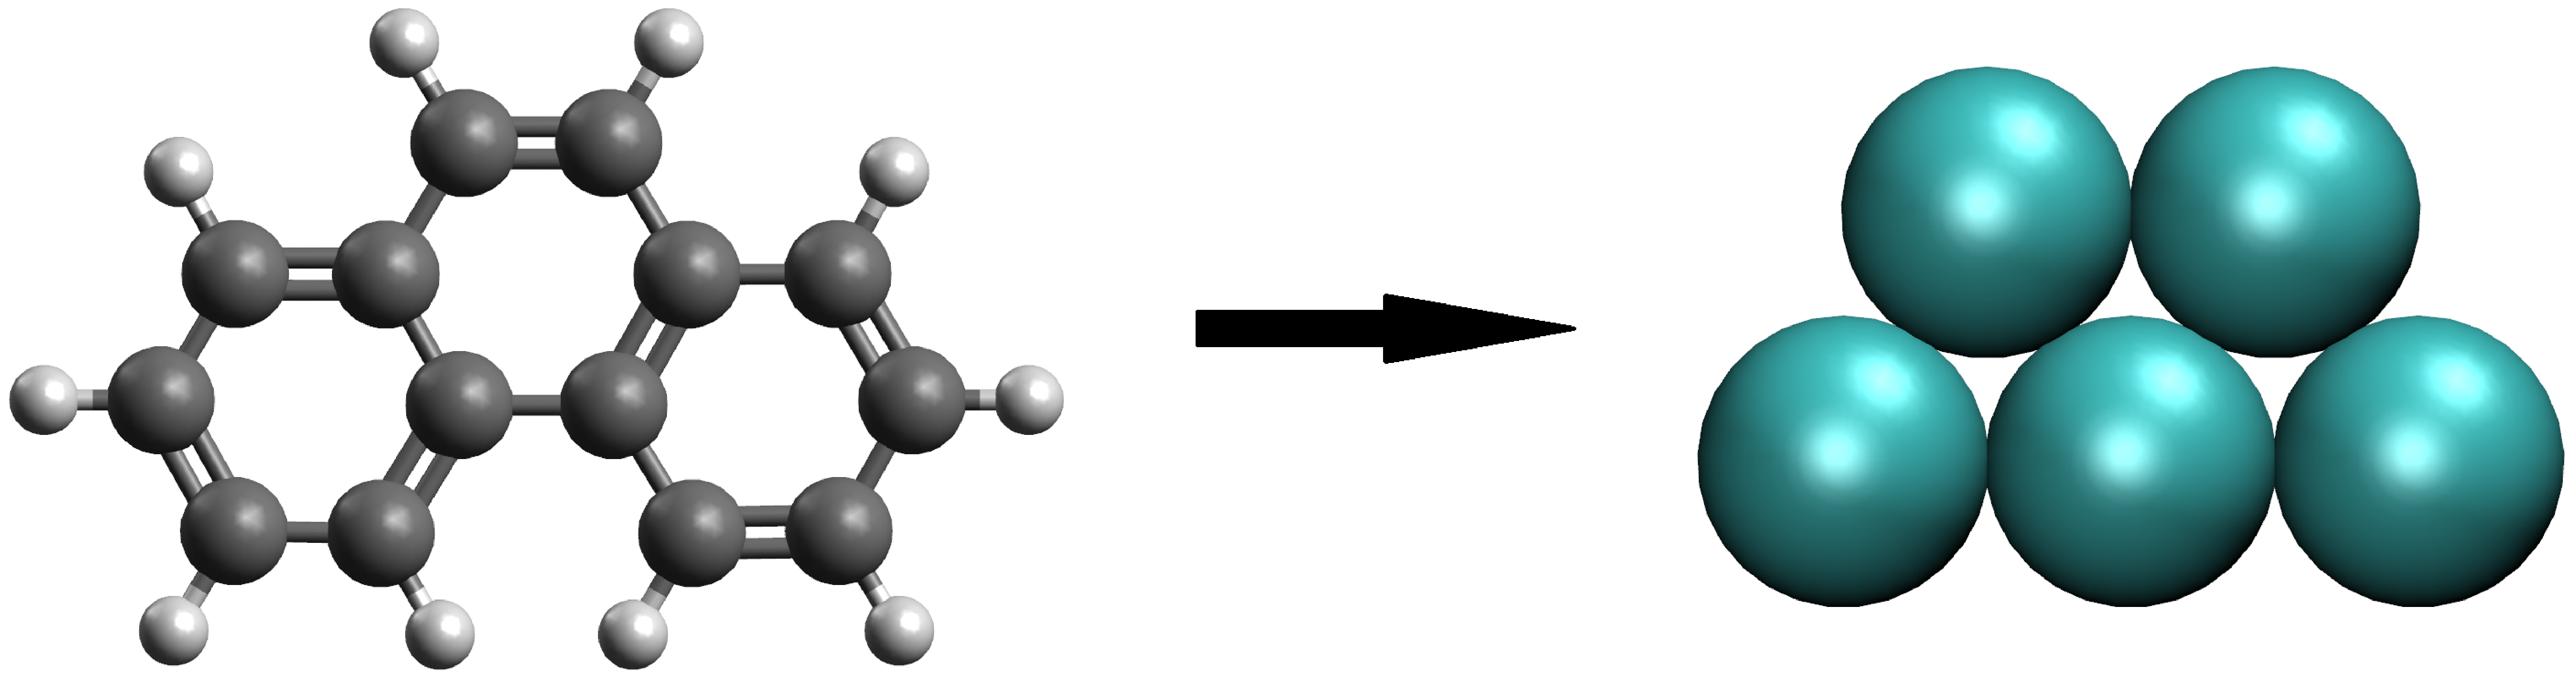
\includegraphics[width=0.9\columnwidth]{Figures/phenanthrene.eps}
		\caption{Level of coarse-graining and geometry chosen for the phenanthrene molecule.}
		\label{fig:fen5}
	\end{figure}
	
	\begin{figure}
		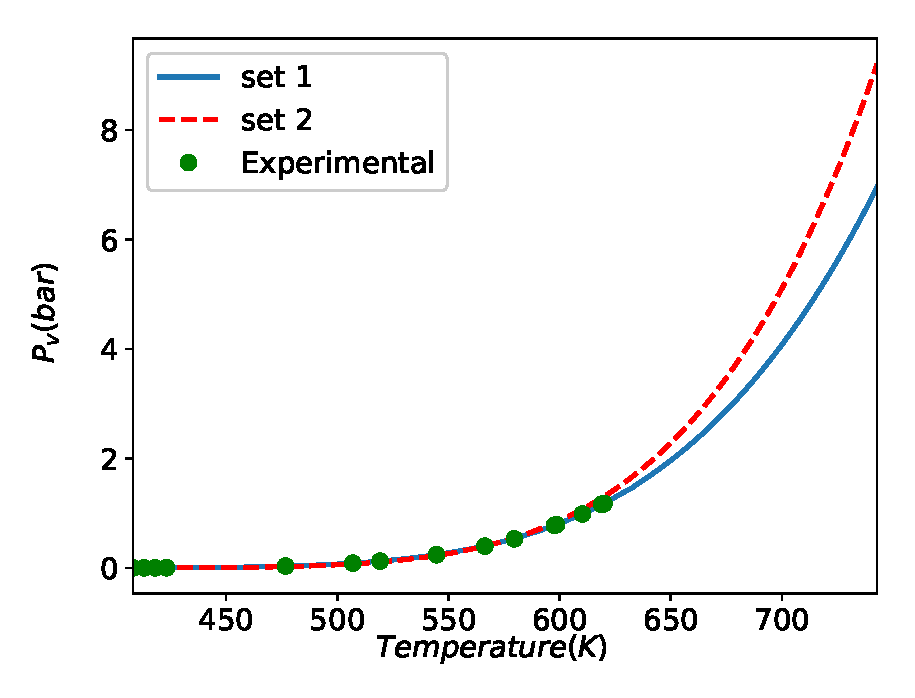
\includegraphics[width=0.9\columnwidth]{Figures/eospv}
		\caption{Vapor pressure of phenanthrene ($P_{v}$) as a function of temperature. The symbols represent experimental data from Refs.~\citenum{murphy} and \citenum{osborn}. The blue curve is a result of calculations using the SAFT-VR Mie EoS with the first set of parameters ($\epsilon/k_b$ = 262.74 K, $\sigma$ = 4.077 \AA, and $\lambda_r$ = 9.55) and the red curve is the result with the second set of parameters ($\epsilon/k_b$ = 350.46 K, $\sigma$ = 3.689 \AA, and $\lambda_r$ = 13.58).}
		\label{fig:edefitpv}
	\end{figure}
	
		\begin{figure}
			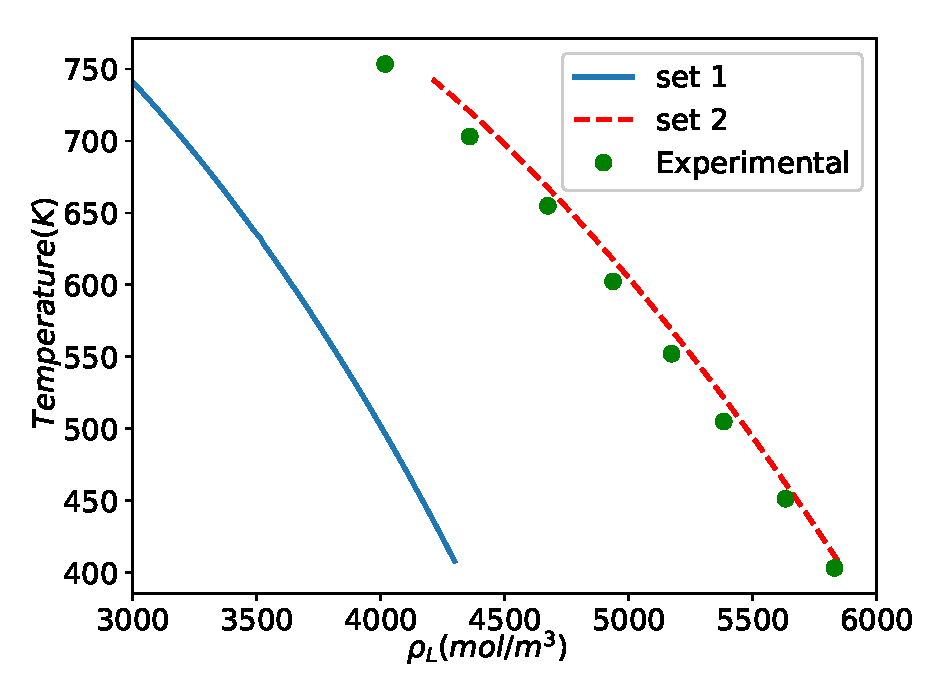
\includegraphics[width=0.9\columnwidth]{Figures/eosdens}
			\caption{Liquid density of phenanthrene ($\rho_{L}$) as a function of temperature. The symbols represent experimental data from NIST \cite{LEMMON-RP91} . The blue curve is a result of calculations using the SAFT-VR Mie EoS with the first set of parameters ($\epsilon/k_b$ = 262.74 K, $\sigma$ = 4.077 \AA, and $\lambda_r$ = 9.55) and the red curve is the result with the second set of parameters ($\epsilon/k_b$ = 350.46 K, $\sigma$ = 3.689 \AA, and $\lambda_r$ = 13.58).}
			\label{fig:edefitdens}
		\end{figure}
	
	The parameters for the other compounds were retrieved from the literature, and all these parameters are displayed in Table~\ref{tbl:parameters}. The use of combining rules is necessary only when modeling a mixture with the SAFT-$\gamma$ Mie force field, since each molecule is composed of equal segments. The mixing rules employed for this force field are \cite{lafitte2013}
	\begin{equation}
	\sigma_{ij} =\frac{\sigma_i+\sigma_j}{2},
	\label{eqn:sigmamix}
	\end{equation}
	\begin{equation}
	\lambda_{k_{ij}} = 3 + \sqrt{(\lambda_{k_i}-3)(\lambda_{k_j}-3)}, \quad k=r,a, \quad \text{and}
	\label{eqn:lambdamix}
	\end{equation}
	\begin{equation}
	\label{eqn:epsmix}
	\epsilon_{ij} =(1-k_{ij})\frac{\sqrt{\sigma_i^3\sigma_j^3}}{\sigma_{ij}^3}\sqrt{\epsilon_i\epsilon_j}.
	\end{equation}
	
	These mixing rules are available in the literature and have been employed in other papers in which this force field was used. In Eq.~\eqref{eqn:epsmix}, $k_{ij}$ is a binary interaction parameter. This parameter accounts for the interactions among chemically distinct compounds, which are not explicitly considered by the SAFT-VR Mie EoS. In our study, the binary interaction parameter was only necessary for aqueous mixtures.
	
	\begin{table}
		\centering
		\caption{SAFT-$\gamma$ Mie force field parameters used for each substance in this work. The well-depth parameter is presented as values of $\epsilon/k_b$ in $K$, where $k_b$ is the Boltzmann constant.}
		\label{tbl:parameters}
		\begin{tabular}{ccccc}
			\hline\hline
			& $m_s$ & $\epsilon/k_{b}$ (K) & $\sigma (\dot{A})$ & $\lambda_r$ \\ \hline
			Water \cite{lobanova2016}        & 1     & 305.21               & 2.902              & 8.0         \\
			Propane \cite{herdes2015}        & 1     & 426.08               & 4.871              & 34.29       \\
			Carbon dioxide \cite{herdes2015} & 2     & 194.94               & 2.848              & 14.65       \\
			Hexane \cite{herdes2015}         & 2     & 376.35               & 4.508              & 19.57       \\
			Octanol \cite{ervik2016}         & 3     & 495.71               & 4.341              & 28.79       \\
			Toluene \cite{muller2017}        & 3     & 268.24               & 3.685              & 11.80       \\
			Benzene \cite{muller2017}        & 3     & 230.30               & 3.441              & 10.45       \\
			Pyrene \cite{muller2017}         & 4     & 459.04               & 4.134              & 15.79       \\
			Anthracene \cite{muller2017}     & 5     & 259.68               & 3.631              & 9.55        \\
			Phenanthrene (set 1)               & 5     & 262.74               & 4.077              & 9.55        \\
			Phenanthrene (set 2)               & 5     & 350.46               & 3.689              & 13.58        \\ \hline\hline
		\end{tabular}
		
	\end{table}
	
	\subsection{Expanded Ensemble}
	\label{sec:expanded ensemble}
	
	The strategy chosen to calculate the solvation free energies was a gradual insertion of the solute molecule in the solvent using an alchemical thermodynamic path \cite{klimovich}. Each alchemical state is represented by the value of a coupling parameter, $\lambda$, which ranges from 0 to 1. When $\lambda=0$, there is no interaction with the solvent and, when $\lambda=1$, the interactions are fully activated. Since the force field used does not explicitly take charges in consideration, the interactions are only due to the Mie potential. For a partial coupling of the Mie potential, we propose a generalized softcore Mie equation based on the model of Beutler \textit{et al}. \cite{beutler}, which is
	\begin{equation}
	\label{eq:miesoftcore}
	\begin{aligned}
	U_{Mie}^{sc}(r) = \lambda C \epsilon \Bigg\lbrace & \frac{1}{\left[\alpha(1-\lambda)+ (r/\sigma)^{\lambda_a}\right]^{\lambda_{r}/\lambda_{a}}} \\ &-\frac{1}{\alpha(1-\lambda)+(r/\sigma)^{\lambda_a}} \Bigg\rbrace,
	\end{aligned}
	\end{equation}
	where $\alpha$ is a constant whose value is normally assumed to be 0.5. Instead of performing various simulations at different alchemical states to obtain the potential energies of Eq.~\eqref{eq:miesoftcore}, we decided to use the Expanded Ensemble method \cite{lyubartsev}, which allows a non-Boltzmann sampling of all states in a single simulation. In this scheme, the sampling is done by biasing the phase space exploration process with weights. The partition function of the expanded ensemble, $Z^{EE}$, is obtained from the probability distributions corresponding to each $\lambda$. It is defined as a weighted sum of subensemble partition functions for discrete values of $\lambda$, that is,
	\begin{equation}
	Z^{EE} = \sum_{i=1}^{N} Z_{i} \exp(\eta_{i}),
	\label{ee}
	\end{equation}
	where $N$ is the number of alchemical states, $\eta_i$ is the arbitrary weight of the subensemble at each state, and $Z_{i}$ is the configurational partition function of state $i$. Here, we followed the flat-histogram approach to calculate the weights \cite{lyubartsev}. This strategy aims to obtain adequate sampling by ensuring that all the states have an equal number of visits, i.e. the probability of sampling state $i$ ($\pi_{i}$) is equal to that of sampling state $j$ ($\pi_{j}$). Using this relation, the following equation can be obtained:
	\begin{equation}
	\label{eqn:weight}
	\eta_{i} - \eta_{j} = \beta (G_i-G_j).
	\end{equation}
	
	Thus, the choice of weights is dependent on the very free energies we are trying to obtain. This equation is then solved iteratively with trial simulations. For the first simulation, the values of $\eta$ are set to zero, and a generally non-flat histogram of state visits is obtained. We then estimate the free energy differences with the MBAR (Multistate Bennett Acceptance Ratio) method \cite{mbar} (see Sec.~\ref{mds}) and, from Eq.~\eqref{eqn:weight}, the next employed set of $\eta$ values are calculated. This iteration goes on until a uniform distribution is attained. The weights found are then used in a longer simulation to obtain the final solvation free energies.
	
	The choice of the $\lambda$ set corresponding to overlapping alchemical states are crucial to the computation of accurate free energy differences. In this work, the method chosen to obtain an optimal staging of the $\lambda$ domain is the one developed by Escobedo and Mart\'{i}nez-Veracoechea \cite{escobedo2007}, based on the study of Katzgraber \textit{et al}. \cite{1742-5468-2006-03-P03018}. This method targets bottlenecks in the simulation by maximizing the number of round trips per CPU time between the lowest ($0$) and highest ($1$) values of $\lambda$. The steady-state flow rate of the simulation, which ``walks'' through the values of $\lambda$, is estimated by a Fick-type diffusion law,
	\begin{equation}
	\phi = D(\Lambda) \Pi (\Lambda) \dfrac{dx(\Lambda)}{d \Lambda},
	\label{eqn:stream}
	\end{equation}
	where $\Lambda$ is the actual, continuous value of the coupling parameter, $D(\Lambda)$ is the diffusivity at state $\Lambda$, $\Pi(\Lambda)$ is the probability density function, and $x(\Lambda)$ is the fraction of times that a simulation, being at state $\Lambda$, has most recently visited the state $\Lambda=1$ as opposed to state $\Lambda=0$. The flow rate $\phi$ is maximized if the probability density $\Pi(\Lambda)$ is proportional to $[D(\Lambda)]^{-1/2}$ \cite{escobedo2007,1742-5468-2006-03-P03018}, where $D(\Lambda)$ can be estimated (up to an additive constant) from Eq.~\eqref{eqn:stream} via finite differences. The optimal $\lambda$ states are then obtained iteratively using the inverse of a cumulative probability $\Phi(\lambda) = \int_0^\lambda \Pi(\Lambda) d\Lambda$. A graphical demonstration of the relation between the new optimized coupling parameters and the cumulative probability is presented in Figure \ref{fig:optimized_cdf}.
	
	\begin{figure}
		\centering
		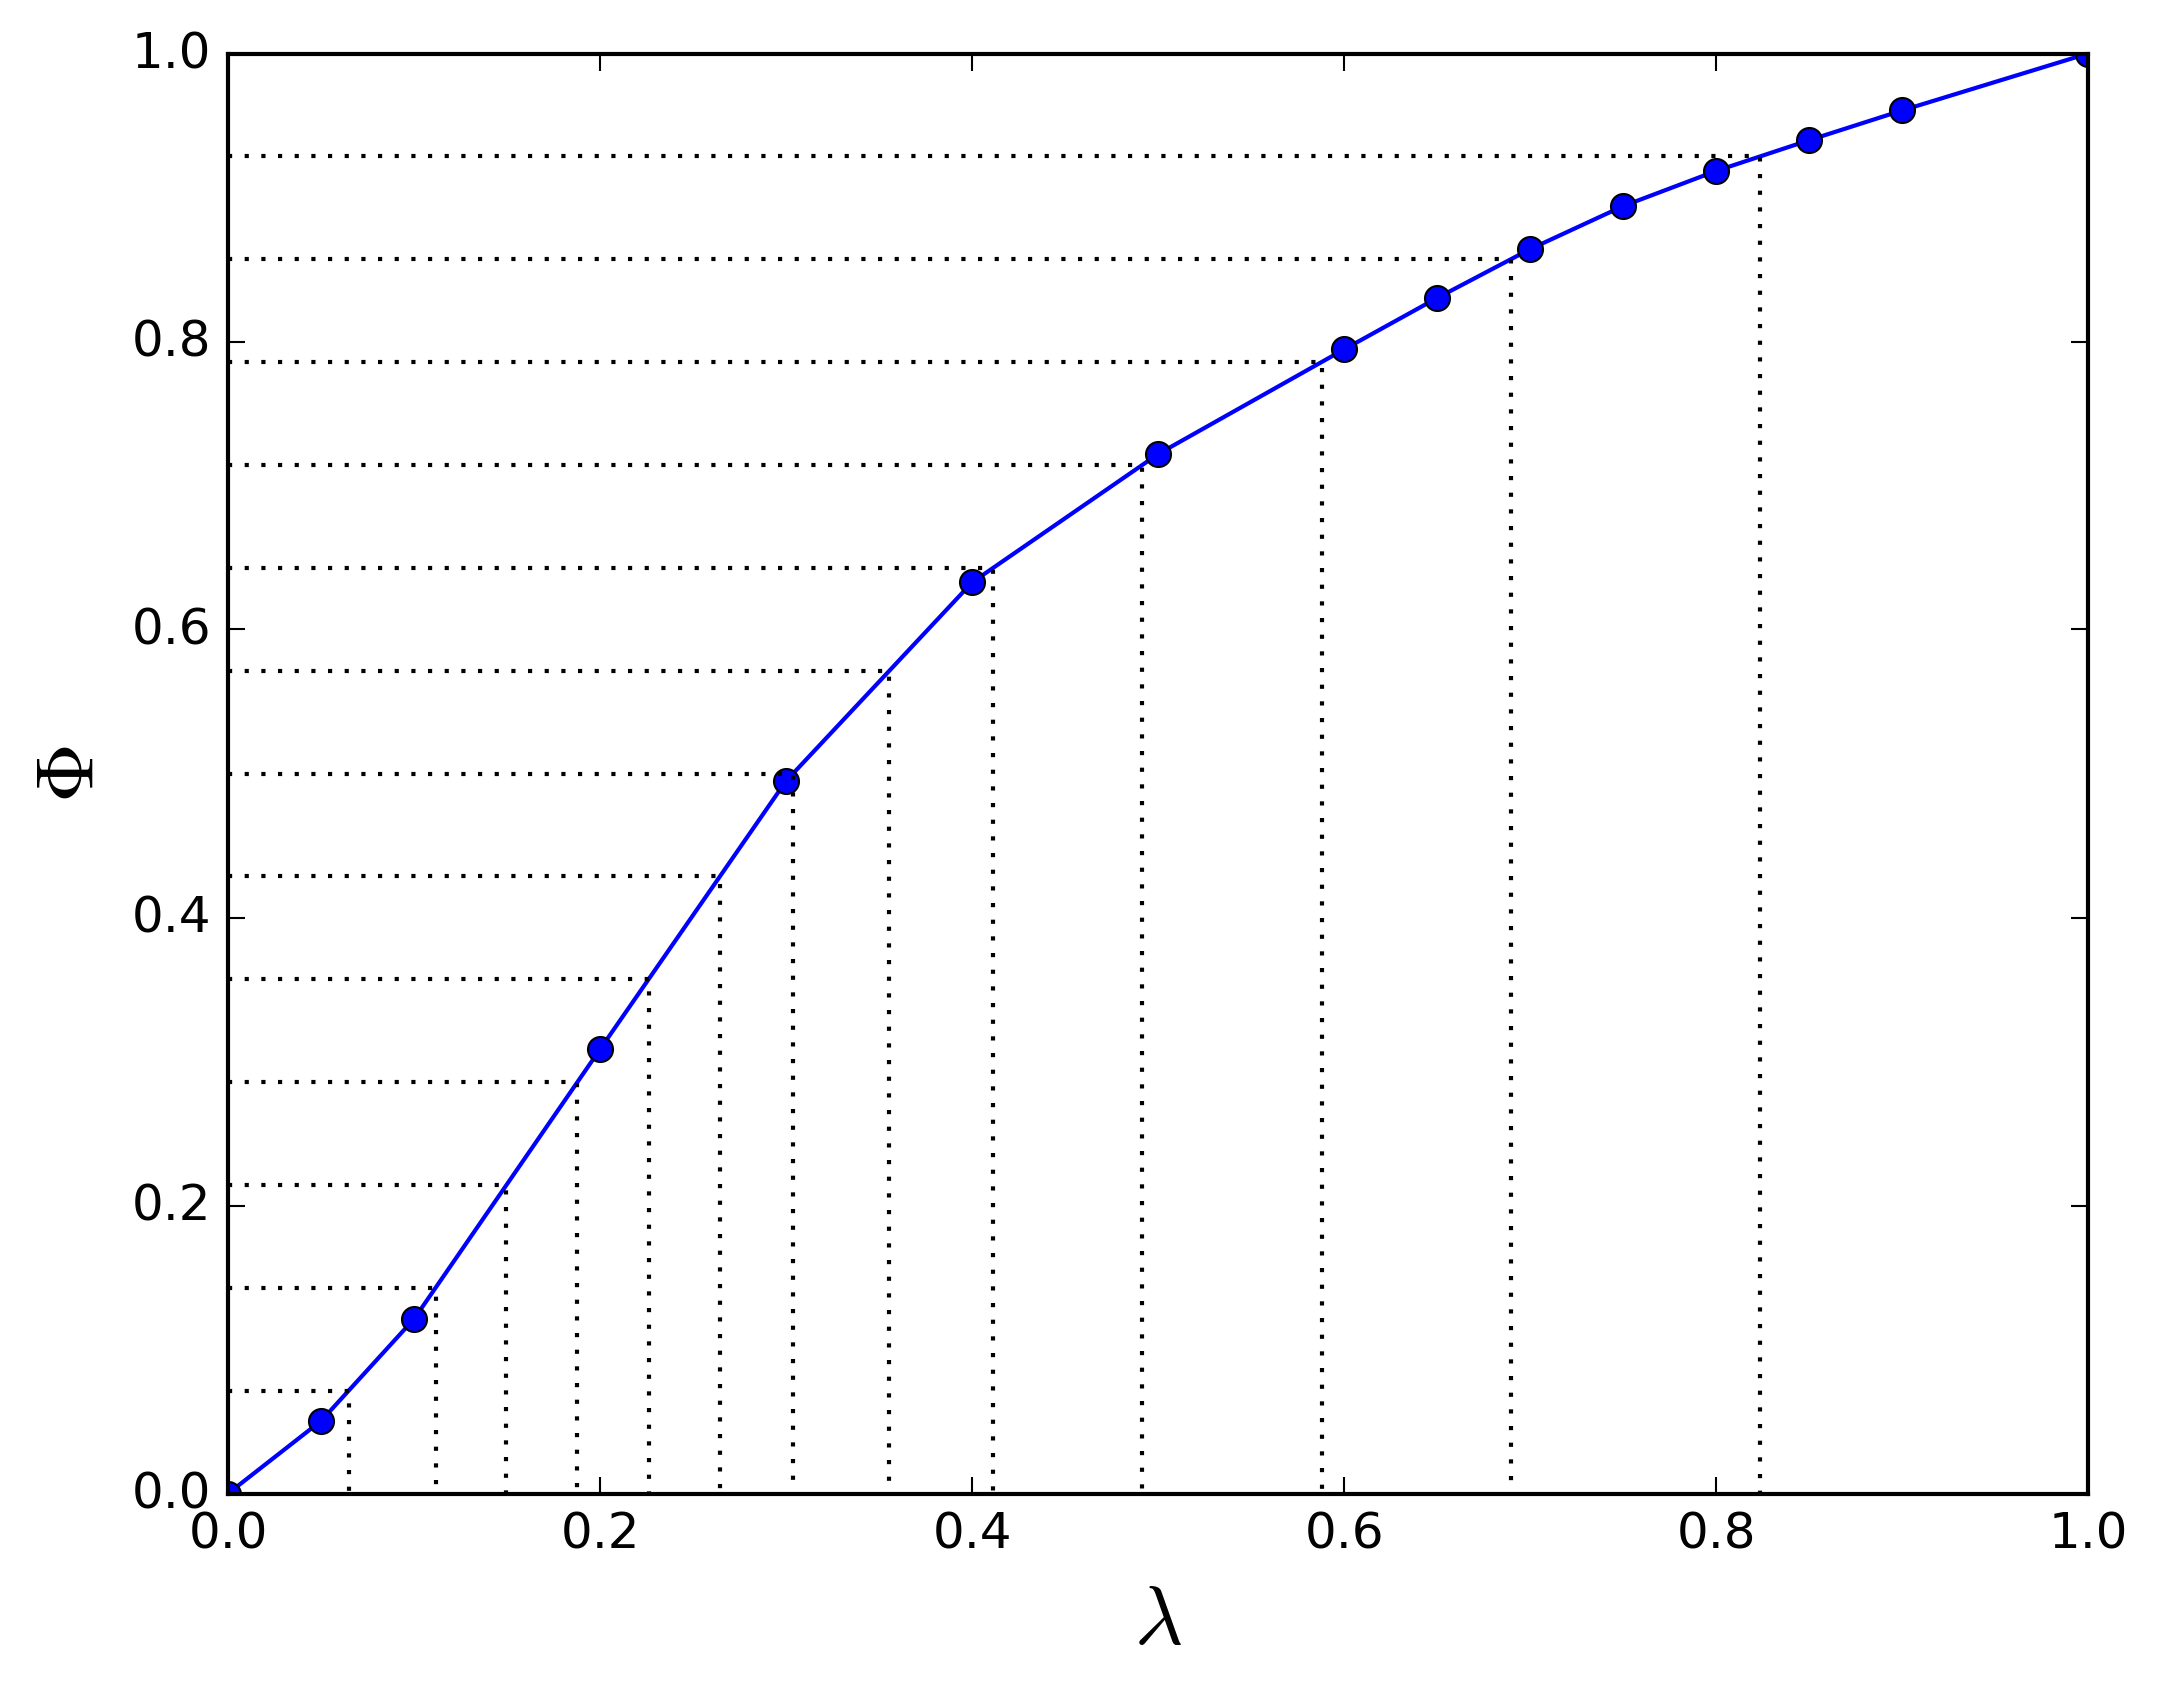
\includegraphics[width=0.9\columnwidth]{Figures/optimized_cdf}
		\caption{Cumulative probability used to obtain the optimized coupling parameter staging for computing the solvation free energy of benzene in hexane using the SAFT-$\gamma$ Mie force field (see Sec.~\ref{sec:non-aqueous}).}
		\label{fig:optimized_cdf}
	\end{figure}
	
	\section{Molecular Dynamics Simulations}\label{mds}
	
	Using the parameters of Table~\ref{tbl:parameters}, we carried out molecular dynamics simulations to obtain samples of potential energies at each expanded ensemble. The software package used to perform the simulations was LAMMPS \cite{lammps}. As required by the coarse-grained model, molecules with more than one segment were treated as rigid bodies. For simulating rigid bodies at constant temperature $T$ and pressure $P$, the algorithm implemented in LAMMPS is that of Kamberaj \textit{et al}. \cite{kamberaj}, in which the translational and rotational degrees of freedom are handled separately by independent Nos\'{e}-Hoover chain thermostats \cite{PhysRevA.31.1695}. All simulations were executed with a time step size of 2~fs, with damping time parameters of 0.2~ps and 2~ps for the thermostats and the barostat, respectively. The potential cutoff distance was set to 20~$\text{\AA}$ \cite{muller2017}, with a neighbor list skin of 2~$\text{\AA}$. The initial configurations of the solvated systems were generated using Playmol \cite{playmol}, which integrates the Packmol package \cite{packmol} with LAMMPS \cite{lammps}. For the binary mixtures, one molecule of solute and a varying number of solvent molecules - 700 of toluene, 700 of octanol, 1024 of hexane, or 3000 of water - were randomly added to a cubic box. In addition to the systems with pure substances acting as solvents, we performed simulations to study the solvation of phenanthrene in a mixture of toluene and carbon dioxide with different weight fractions of \ce{CO_2} ($w_\text{\ce{CO_2}}$). The system consisted of one molecule of phenanthrene for all the cases and 123 molecules of \ce{CO_2} and 618 molecules of toluene ($w_\text{\ce{CO_2}} = 0.087$); 166 molecules of \ce{CO_2} and 589 molecules of toluene ($w_\text{\ce{CO_2}} = 0.119$); 232 molecules of \ce{CO_2} and 545 molecules of toluene ($w_\text{\ce{CO_2}} = 0.169)$; 380 molecules of \ce{CO_2} and 446 molecules of toluene ($w_\text{\ce{CO_2}} = 0.289$).
	
	All simulations were performed at constant temperature and pressure values of 298 K and 1 bar, respectively, except the ones for systems containing carbon dioxide. These ones were performed at the temperature of 298 K and at the experimental bubble-point pressure reported in Ref.~\cite{co2toliq} for each considered liquid-phase composition. For all simulations, the initial box was equilibrated in the NPT ensemble for 2~ns with the solute molecule totally coupled to the system (i.e. $\lambda = 1$), and the final configurations were used as the initial conditions for the expanded ensemble simulations. These were carried out with a LAMMPS package developed by our research group for expanded ensemble simulations, named USER-ALCHEMICAL and available at \url{github.com/atoms-ufrj}.
	
	During the expanded ensemble simulations, the sampling of a new alchemical state was tried at every 10 MD steps. To define the optimal values of $\lambda$ and $\eta$ corresponding to each state, relatively large trial simulations, having around 9 ns of production time, were carried out in order to ensure an adequate sampling of the intermediate states. In the first simulation, we chose a group of 15 equally-spaced $\lambda$ values, and we either set all $\eta$ values to zero or assigned values previously found for similar solute-solvent pairs. The subsequent $\eta$ sets were estimated with the flat-histogram approach expressed by Eq.~\eqref{eqn:weight}. We then performed another trial simulation with the new weights. The results of this simulation were used to optimize the $\lambda$ staging such as described in Sec.~\ref{sec:expanded ensemble}. The $\eta$ values corresponding to the newest $\lambda$ staging were interpolated linearly from the free energy differences. With the final values of $\eta$ and $\lambda$ defined for each mixture, larger simulations with a production time of 20 ns were carried out.
	
	Since the employed force field does not explicitly includes point charges in the molecular segments, the only contribution to the total potential energy of the inserted solute molecule is due to the softcore potential of Eq.~\eqref{eq:miesoftcore}. The post-processing method used to effectively calculate free-energy differences with the potential energies obtained from the expanded ensemble simulations was the Multistate Bennett Acceptance Ratio (MBAR) method \cite{mbar}. A software developed by Klimovich \textit{et al}. \cite{klimovich} for alchemical calculation analysis was used to obtain the values of $\Delta G_\text{solv}$ with MBAR and to assess the quality of the results.
	
	After the first estimations, we realized that the binary interaction parameter of Eq.~\eqref{eqn:epsmix} was necessary for systems having water as a solvent. Hence, we estimated $k_{ij}$ for these pairs only (for all the other pairs, we have set $k_{ij}$ to zero). The estimation was done by performing trial expanded ensemble simulations with three distinct values of $k_{ij}$, as suggested by Ervik \textit{et al}. \cite{ervik20162}. With the values of $\Delta G_\text{solv}$ obtained from these simulations, we carried out a linear fit and comparison to experimental data \cite{P29900000291, doi:10.1021/ct050097l} in order to obtain the refined value of the parameter. We used this strategy because the estimation of $k_{ij}$ using a top-down approach with the SAFT-VR Mie EoS gave poor results for the hydration free energies.
	
	\section{Results and discussion}
	\label{sec:results}
	
	\subsection{Solvation free energies in non-aqueous solvents}
	\label{sec:non-aqueous}
	
	Our primary intention with this study is to assess the capability of the SAFT-$\gamma$ Mie force field to yield solvation free energies. For this, we have chosen benchmark solutes used in the literature (benzene and propane) and aromatic solutes (benzene, pyrene, phenanthrene, and anthracene), as well as non-polar (hexane), aromatic (toluene), and hydrogen-bonding (1-octanol and water) solvents. The solvation free energy simulations for the chosen solute-solvent pairs were carried out with binary interaction parameters set equal to zero since these parameters were not necessary according to our preliminary studies. For the solvation free energy of phenanthrene, the calculations were done for both set of parameters of Table \ref{tbl:parameters}.  As the force field does not explicitly account for charges, we only calculated the Mie contribution (Eq.~\eqref{eq:miesoftcore}) to the solvation free energy. A total of 15 to 18 $\lambda$ values, depending on the solute-solvent pairs, and their respective $\eta$ weights were estimated as described in the previous sections. The final $\lambda$ set for every pair was found using the cumulative probability distribution mentioned in Sec.~\ref{sec:expanded ensemble}. For the benzene/hexane case, such probability distribution can be seen in Fig.~\ref{fig:optimized_cdf}. Here and henceforth, we employ the terminology solute/solvent (in this order) to refer to the simulated pairs. The optimized values of $\lambda$ and $\eta$ for all pairs are provided in Tables S1 to S4 as supplementary material.
	After the expanded ensemble simulations with the optimized intermediate states and weights, we calculated the solvation free energies with MBAR. The results obtained and the absolute deviations from experimental data \cite{doi:10.1021/ci034120c} are available in Table~\ref{tbl:solv1}. The absolute deviations of the solvation free energies in hexane were smaller than the deviations in other solvents. Comparing the phenanthrene solvation free energies of phenanthrene calculated with both set of parameters, we observe that set 2, which was estimated with liquid density, had a  smaller absolute deviation.
	Additionally, the SAFT-$\gamma$ Mie force field presented better results for benzene/hexane than the TraPPE ($- 4.35 \pm 0.05$ kcal/mol, from Ref.~\citenum{garrido2011}) and the ELBA ($-2.92 \pm 0.01$ kcal/mol, from Ref.~\citenum{doi:10.1021/acs.jctc.5b00963}) force fields.
	TraPPE is a force field parametrized with fluid-phase equilibrium data that uses the Lennard-Jones potential to describe the non-bonded interactions. In Ref.~\citenum{garrido2011}, the authors used the united-atom description of the TraPPE force field for the alkyl group, the all-atom description for the polar groups and the explicit-hydrogen approach for the aromatic groups. In the explicit-hydrogen approach, the interaction sites for all hydrogen atoms, some lone pair electrons, and bond centers are accounted for \cite{doi:10.1021/jp073586l}. In turn, the ELBA force field is a coarse-grained model that comprises Lennard-Jones parameters ($\sigma$ and $\epsilon$), bonded parameters, and dipole moments for polar beads. This force field models three carbon atoms as one Lennard-Jones site and one water molecule as a single Lennard Jones site with a point-dipole. We also present the solvation free energies corresponding to each alchemical state ($\lambda$) for all the solute/solvent pairs studied here in Figures \ref{fig:hex} to \ref{fig:tol}. Observing the solvation free energy in hexane (Fig.~\ref{fig:hex}) specifically, we can note the effect of molecule size (pyrene $>$ phenanthrene $>$ benzene) on the region of the free energy curve corresponding to the first values of $\lambda$ where the cavity required for inserting the solute is formed.
	
	\begin{table*}
		\centering
		\caption{Solvation free energies (kcal/mol) in non-aqueous solvents calculated with the SAFT-$\gamma$ force field and experimental data.}
		\label{tbl:solv1}
		\begin{tabular}{cccccc}
			\hline\hline
			Solute       & Solvent   & $\Delta G_\text{solv}^\text{exp}$ & $\Delta G_\text{solv}^\text{Mie}$ & Abs. Dev.  \\ \hline
			benzene      & hexane    & -3.96                   & -3.76  $\,$ $\pm$ 0.01       & 0.20      &  \\
			pyrene       & hexane    & -11.53                  & -10.82 $\pm$ 0.02       & 0.71      &  \\
			phenanthrene(set 1) & hexane    & -10.01                  & -9.16  $\,$ $\pm$ 0.01       & 0.85      &  \\
			phenanthrene(set 2) & hexane    & -10.01                  & -9.63  $\,$ $\pm$ 0.01       & 0.38     &  \\
			propane      & 1-octanol & -1.32                   & -1.36  $\,$ $\pm$ 0.03       & 0.04      &  \\
			anthracene   & 1-octanol & -11.72                  & -8.12   $\,$ $\pm$ 0.03       & 3.61      &  \\
			phenanthrene(set 1) & 1-octanol & -10.22                  & -8.34  $\,$ $\pm$ 0.03       & 1.88      &  \\
			phenanthrene(set 2) & 1-octanol & -10.22                  & -9.97  $\,$ $\pm$ 0.03       & 0.24     &  \\			
			pyrene       & toluene   & -12.86                  & -11.74 $\pm$ 0.01       & 1.11      &  \\
			anthracene   & toluene   & -11.31                  & -9.90 $\,$ $\pm$ 0.01        & 1.41      &  \\ 
			phenanthrene(set 1)   & toluene   & -                  & -10.65 $\pm$ 0.02      & -     &  \\ 
			phenanthrene(set 2)   & toluene   & -                  & -10.79	 $\pm$  0.01        & -      &  \\ 
			\hline\hline
			&
		\end{tabular}
	\end{table*}
	\begin{figure}
		\centering
		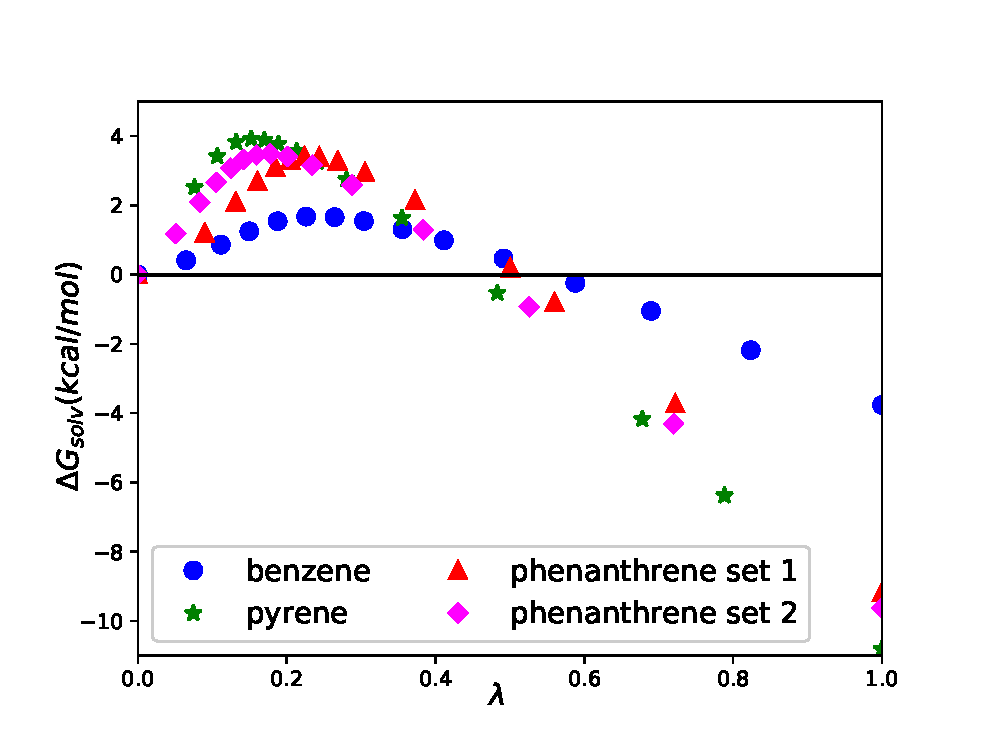
\includegraphics[width=1.0\linewidth]{Figures/hexartsets.eps}
		\caption{Representation of solvation free energies of different solutes in hexane calculated using the SAFT-$\gamma$ Mie force field. Each point on the graph represents the solvation free energy difference estimated with MBAR at each alchemical state.}
		\label{fig:hex}
	\end{figure}
	\begin{figure}
		\centering
		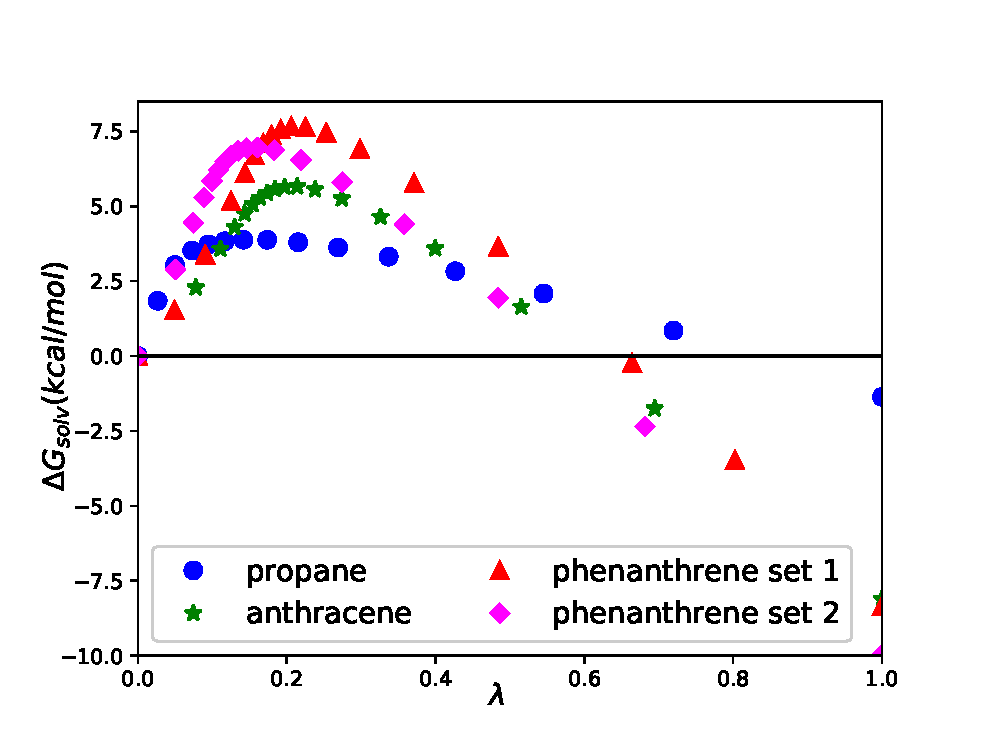
\includegraphics[width=1.0\linewidth]{Figures/octartsets.eps}
		\caption{Representation of solvation free energies of different solutes in 1-octanol calculated using the SAFT-$\gamma$ Mie force field. Each point on the graph represents the solvation free energy difference estimated with MBAR at each alchemical state.}
		\label{fig:oct}
	\end{figure}
	\begin{figure}
		\centering
		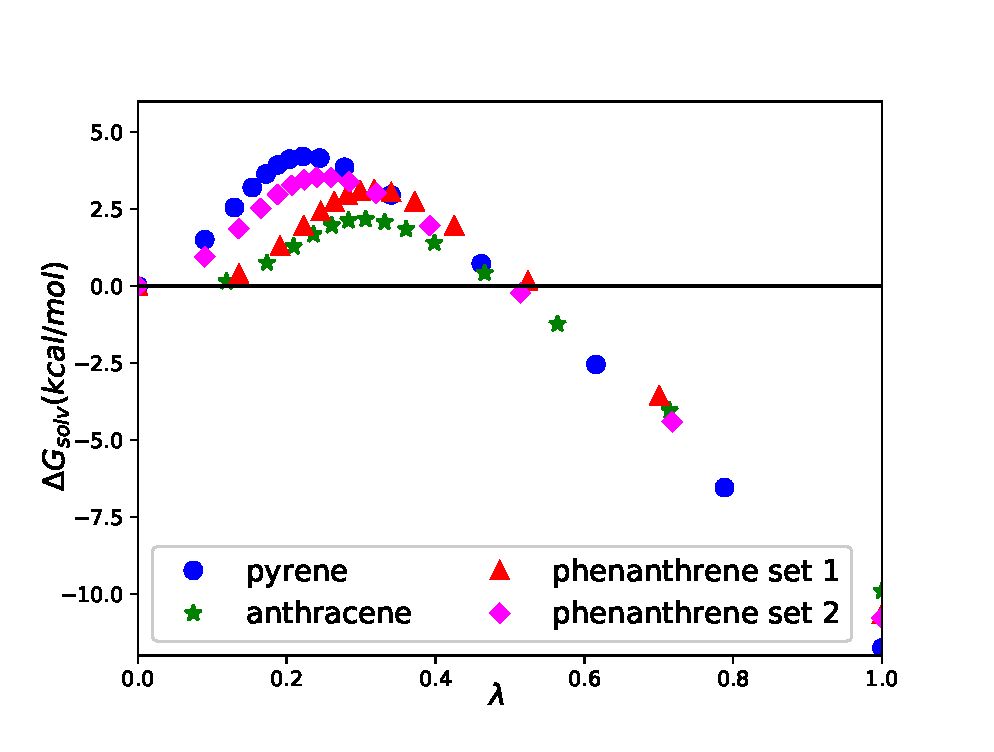
\includegraphics[width=1.0\linewidth]{Figures/tolartsets.eps}
		\caption{Representation of solvation free energies of different solutes in toluene calculated using the SAFT-$\gamma$ Mie force field. Each point on the graph represents the solvation free energy difference estimated with MBAR at each alchemical state. }
		\label{fig:tol}
	\end{figure}
	
	The solvation free energies of propane and phenanthrene in 1-octanol with the both sets of parameters lied in the desired deviation range of 1-2 kcal/mol \cite{doimobley}. We also highlight the decrease in the absolute deviation of the solvation free energy of phenanthrene when the set 2 of parameter is used.For propane, the observed deviation in solvation free energies was much smaller when compared to the other solutes, which can possibly be attributed to the non-polarity of propane and its smoother free energy curve, presented in Fig.~\ref{fig:oct}. This deviation is also smaller than that obtained with the ELBA force field for the propane/1-octanol system ($-0.92 \pm 0.01$ kcal/mol, from Ref.~\citenum{doi:10.1021/acs.jctc.5b00963}). The absolute deviation of the solvation free energy computed for anthracene/1-octanol is much higher than that calculated for phenanthrene/1-octanol. Despite the structural difference of anthracene and phenanthrene, their molecules are modeled with the same geometry (Fig.~\ref{fig:fen5}) in the SAFT-$\gamma$ Mie force field. The high deviation observed for the solvation free energy of anthracene in 1-octanol might indicate that the chosen geometry is not adequate for anthracene, thus highlighting the importance of molecular geometry for this force field.
	Another possible reason is the acentric factor value ($\omega=0.3314$) used in Ref.~\citenum{muller2017} to obtain the Mie parameters of anthracene.
	%This property plays a crucial role in their proposed correlation, since it determines the repulsive term exponent of the Mie potential, which then affects the other parameters.
	With an Antoine-model fitting of vapor pressure data \cite{murphy}, followed by extrapolation up to $T_c$ (the critical temperature) \cite{muller2017} and evaluation at $T/T_c=0.7$, we managed to obtain $\omega=0.473$.
	Another value found in the literature \cite{poling2000properties} for the acentric factor of this compound is $\omega=0.501$.
	Note that both values are way above $0.3314$.
	This discrepancy seems odd and deserves further investigation, but this is beyond the scope of the present work.

	The results also indicate a reasonable capability of the force field for predicting the solvation free energies of polyaromatic solutes in aromatic solvents. The influence of the molecular geometry on the solvation free energy curves was the same as the one observed for other solvents, as can be seen in Fig.~\ref{fig:tol}. We also calculated the $\Delta G_{solv}$ for phenanthrene in pure toluene and in toluene+\ce{CO_2} mixtures. From Table \ref{tbl:solv1}, we note that difference between the solvation free energy of phenanthrene calculated with the two sets of parameters is small. As far as we were able to verify, there are no available experimental data for these solvation free energies, but the previous results for phenanthrene in other solvents showed that the force field is adequate to describe the solvation phenomenon of phenanthrene in a pure aromatic solvent. Hence, we decided to carry out a qualitative study of the influence of \ce{CO_2} in the solvation free energies of phenanthrene in toluene in order to evaluate the description of this system with the SAFT-$\gamma$ Mie force field. The results of these test sets are shown in Table~\ref{tbl:solvco2}. The increase of the mass fraction of \ce{CO_2} in toluene caused a small effect on the solvation free energies in the range of weight fractions (0.087-0.289) studied here. First, the $\Delta G_\text{solv}$ decreased with the increase of $w_\text{\ce{CO_2}}$ up to 0.119. After that, the effect was reversed, and carbon dioxide became an anti-solvent. Soroush \textit{et al}. \cite{SOROUSH2014405} reported that asphaltene precipitation occurs when carbon dioxide mass fractions became higher than 0.10 in the system asphaltene+toluene+\ce{CO_2}, which is in agreement with the observed anti-solvent effect of carbon dioxide. Nevertheless, the differences observed here are small. These minor differences may indicate that the effect of \ce{CO_2} is negligible in the solvation of phenanthrene in toluene modeled with the SAFT-$\gamma$ Mie force field. Additional studies are needed to make a safe assertion about it. It is also worth remarking that this is a qualitative study due to the lack of experimental data. Overall, the methodology proposed by the SAFT-$\gamma$ Mie force field was satisfactory in predicting the solvation free energies of the solute-solvent pairs studied here.
	
	\begin{table}
		\centering
		\caption{Calculated values for the solvation free energies (kcal/mol) of phenanthrene in toluene+\ce{CO_2}.}
		\label{tbl:solvco2}
		\begin{tabular}{ll}
			\hline\hline
			$w_\text{\ce{CO_2}}$ & $\Delta G_{solv}^{Mie}$ \\ \hline
			0.0          & -10.65 $\pm$ 0.02       \\
			0.087        & -10.73 $\pm$ 0.02       \\
			0.119        & -10.78 $\pm$ 0.02       \\
			0.169        & -10.71 $\pm$ 0.02       \\
			0.289        & -10.69 $\pm$ 0.02       \\ \hline\hline
		\end{tabular}
	\end{table}
	
	\subsection{Hydration free energies}
	
	Water is a solvent extensively used in experimental and computational studies.
	Because of this importance and the fact that water has unique properties, such as density maximum at 277 K and increased diffusivity upon compression, developing an accurate computational model for water is an ongoing quest \cite{hadley2012}.
	Hence, we also calculated the solvation free energies in water (hydration free energies) with the SAFT-$\gamma$ Mie force field.
	With these calculations, we intend to verify whether this coarse-grained model would represent the water molecule correctly and be a good alternative for decreasing the computational cost of solvation studies with asphaltene-like models.
	The simulations with water as a solvent were carried out using widely studied solutes, either aliphatic (propane) or aromatic (benzene, toluene, and phenanthrene) ones.
	A set of fifteen intermediate $\lambda$ states was considered in each case.
	These $\lambda$ values and their corresponding $\eta$ weights, obtained with the methodology explained in Sec.~\ref{sec:expanded ensemble}, are available in the supplementary material (Table S5).
	At first, we set to zero the binary interaction parameters of all aqueous mixtures, but preliminary results for hydration free energies, displayed in Table~\ref{tbl:solv2}, exhibited a high deviation from experimental data \cite{P29900000291, doi:10.1021/ct050097l}.
	With these results, the need for binary interaction parameters became clear.
	In an initial attempt to obtain better results, we estimated $k_{ij}$ following the strategy inherent to the SAFT-$\gamma$ Mie force field of using the SAFT-VR Mie equation of state and experimental vapor-liquid phase equilibrium data.
	However, this strategy also provided results with high absolute deviations from the solvation free energy data.
	Therefore, we decided to use molecular dynamics simulations for estimating $k_{ij}$, such as described in the last paragraph of Sec.~\ref{mds}.
	After finding individual values for the interaction parameter of each pair, we noticed that the values corresponding to aromatic solutes were very similar to each other.
	Thus, we decided to employ a unique, averaged parameter for all aromatic solutes in water.
	We present this general aromatic/water interaction parameter in Table~\ref{tbl:kij}, where one can also find the binary interaction parameter for the propane/water pair.
	
	\begin{table*}
			\centering
			\caption{Hydration free energies (kcal/mol) calculated with the SAFT-$\gamma$ Mie force field and binary interaction parameters.}
			\label{tbl:solv2}
			\begin{tabular}{cccccc}
				\hline\hline
				Solute & $\Delta G_{solv}^{exp}$ & \vtop{\hbox{\strut $\Delta G_{solv}^{Mie}$}\hbox{\strut $k_{ij} = 0$}} & \vtop{\hbox{\strut Absolute}\hbox{\strut Deviation}} & \vtop{\hbox{\strut $\Delta G_{solv}^{Mie}$}\hbox{\strut $k_{ij} \neq 0$}} & \vtop{\hbox{\strut Absolute}\hbox{\strut Deviation}} \\ \hline
				propane & $2.00 \pm 0.20$ & $1.10 \pm 0.01$ & 0.90 & $2.01 \pm 0.01$ & 0.01 \\
				benzene & $-0.86 \pm 0.20$ & $-4.45 \pm 0.03$ &  3.59 & $-1.12 \pm 0.01$ & 0.26 \\
				toluene & $-0.83 \pm 0.20$ & $-10.98 \pm 0.30$ &  10.15 & $-0.84 \pm 0.01$ & 0.01 \\
				phenanthrene (set 1)& $-3.88 \pm 0.60$ & $-10.90 \pm 0.04$ & 7.12 & $-3.47 \pm 0.02$ & 0.41 \\
				phenanthrene (set 2)& $-3.88 \pm 0.60$ & $-10.90 \pm 0.04$ & 7.12 & $-5.12 \pm 0.02$ & 1.24 \\
				\hline\hline
			\end{tabular}
	\end{table*}
	
	\begin{table}
		\centering
		\caption{Estimated binary interaction parameters of Eq. \ref{eqn:epsmix} for aqueous mixtures.}
		\label{tbl:kij}
		\begin{tabular}{cc}
			\hline\hline
			Pair              & $k_{ij}$ \\ \hline
			propane/water  & 0.067    \\
			aromatic/water & 0.154    \\ \hline\hline
		\end{tabular}
	\end{table}
	
	The relatively large $k_{ij}$ value for the interaction between aromatic solutes and water can be related to the lack of an explicit term in the SAFT-$\gamma$ Mie model to account for associations such as hydrogen bonds.
	This is so because the associative term of the SAFT-VR Mie EoS \cite{lafitte2013} has not been incorporated to the force field.
	The SAFT-$\gamma$ Mie model for water has two different temperature-dependent sets of parameters \cite{lobanova2016}.
	In this work, we used the set estimated from experimental interfacial tension data.
	It is worth noting that we have tested the only binary interaction parameter for toluene/water available in the literature \cite{herdes2017}, estimated with MD interfacial data as well.
	Nevertheless, the result once again exhibited a high absolute deviation.
	In other words, this parameter could not be transferred to the calculation of the solvation free energy of toluene in water.
	
	The issues faced by the SAFT-$\gamma$ Mie model can also be related to the problems of modeling water with a coarse-grained force field.
	One of the main difficulties is the choice of how many water molecules are going to be represented by a single bead since water molecules move independently and have non-bonded interactions with each other \cite{hadley2010,hadley2012}.
	The SAFT-$\gamma$ Mie water has one bead per molecule.
	This strategy only saves a small amount of simulation time, but it can predict properties at physiological temperatures unlike other models with more aggressive coarse-graining, such as the MARTINI model, which considers that one bead represents four water molecules.
	In light of all these problems related to modeling the water molecule, the SAFT-$\gamma$ Mie force field appears to be a good alternative when working close to room temperatures.
	However, the necessity of using molecular simulation to estimate additional parameters spotlights a flaw in its top-down methodology.
	The binary parameter estimation increased significantly the simulation time required to calculate the hydration free energies.
	Note that we had to carry out three simulations for every solute/water pair in order to fit the parameters and, in the end, one additional simulation for every pair in order to check the validity of using an averaged parameter for all pairs.
	If these simulations are necessary every time a new mixture with water is modeled with the SAFT-$\gamma$ Mie force field, then its most appealing feature (i.e. practicality) is lost.
	With this in mind, a useful investigation would be to determine to which extent other aromatic/water mixtures can be modeled using the binary interaction parameter estimated here.
	
	Using the binary interaction parameters calculated with data from molecular dynamics, we then obtained the final hydration free energies presented in Table~\ref{tbl:solv2}.
	
	Hydration free energies calculated using the SAFT-$\gamma$ Mie force field with $k_{ij} \neq 0$ had low absolute deviations from the experimental data, as expected since the parameters were adjusted to fit them. Contrary to what happened to the solvation free energy of phenanthrene in the previous section, the hydration free energy of phenanthrene calculated with the second set  had higher absolute deviations than the ones calculated with the first set. This can be due to the fact that we used a global $k_{ij}$ to perform these calculations and the well parameter ($\epsilon / k_b$) of the phenanthrene first set of parameters is more similar to the well parameters of the other aromatic compounds. 	Hydration free energies have also been calculated for the pairs studied here by Genheden \cite{doi:10.1021/acs.jctc.5b00963} with the ELBA force field and by Mobley and Guthrie \cite{PMID:24928188} with the GAFF and TIP3P force fields for the solutes and for water, respectively.
	GAFF (General Amber Force Field) is an all-atom model that consists of bonded and non-bonded parameters and is suitable for the study of a significant number of molecules.
	In turn, TIP3P considers that water is a rigid molecule represented by three point-charge sites, with the one representing the oxygen atom also engaging in van der Waals interactions \cite{doi:10.1063/1.445869}.
	Both GAFF and TIP3P entail the use of the Lennard-Jones potential in the calculation of non-bonded interactions.
	
	Comparing the three aforementioned force fields, the root mean square error (RMSE) of the hydration free energies of propane, benzene, toluene, and phenanthrene (set 1) tested with the SAFT-$\gamma$ Mie model was 0.24, the RMSE for hydration free energies obtained with the GAFF force field was 0.73, and that for the ELBA coarse-grained force field was 0.44.
	The difference between the results of GAFF ($-5.26 \pm 0.03$) and SAFT-$\gamma$ Mie force field with the first set of parameters ($-3.47 \pm 0.02$) is significantly high for phenanthrene, hence the coarse-grained force field with a binary parameter estimated with hydration free energy data is preferred as far as accuracy is concerned.
	The results also indicated that the SAFT-$\gamma$ Mie model performed better than the ELBA force field in modeling the solvation of the pairs studied in this work, but only if the binary interaction parameter is taken into account.This occurred despite the fact that both the SAFT-$\gamma$ Mie and ELBA models have the same level of coarse-graining for the solvent (one bead represents one water molecule).
	Therefore, the best choice between the two coarse-grained models will probably depend on the availability and transferability of binary interaction parameters for the SAFT-$\gamma$ Mie model.
	This study consisted in the calculation of solvation free energies of aromatic solutes in different solvents by using the SAFT-$\gamma$ Mie coarse-grained force field.
	Solvation free energy studies are mostly presented in the literature using water as a solvent and with all-atom force fields based on the Lennard-Jones potential.
	In contrast, in the present study, we provide data about the capability of a coarse-grained force field based on the Mie potential in calculating solvation free energies.
	Additionally, the solvation free energy estimations carried out here can help improve the SAFT-$\gamma$ Mie force field since these calculations are helpful in identifying errors and shortcomings in the modeling process.
	This force field uses the SAFT-VR Mie equation of state in its parameterization, which results in a relatively straightforward top-down method of obtaining parameters.
	Following this strategy, parameters for phenanthrene (which were not reported in the reference paper \cite{muller2017}) were obtained here using vapor pressure (set 1) data and the corresponding states parametrization (set 2).

	In Fig.~\ref{fig:water} we present, for the SAFT-$\gamma$ Mie force field, the hydration free energy of each solvent as a function of the coupling parameter $\lambda$.
	As one can observe, larger molecules exhibit steeper free energy profiles, such as shown for the solvation free energy study in non-aqueous solvents.
	We also observe that the hydration free energy corresponding to the first non-zero value of $\lambda$ is negative for benzene, toluene, and phenanthrene when a positive value is expected since free energy is required for cavity formation in the solvent for the insertion of the solute.
	Determining the cause of this anomaly (whether it stems from the Mie potential parameters, the molecule geometry, or the binary interaction parameter) requires a deeper investigation that is beyond the scope of this article.
	
	\begin{figure}
		\centering
		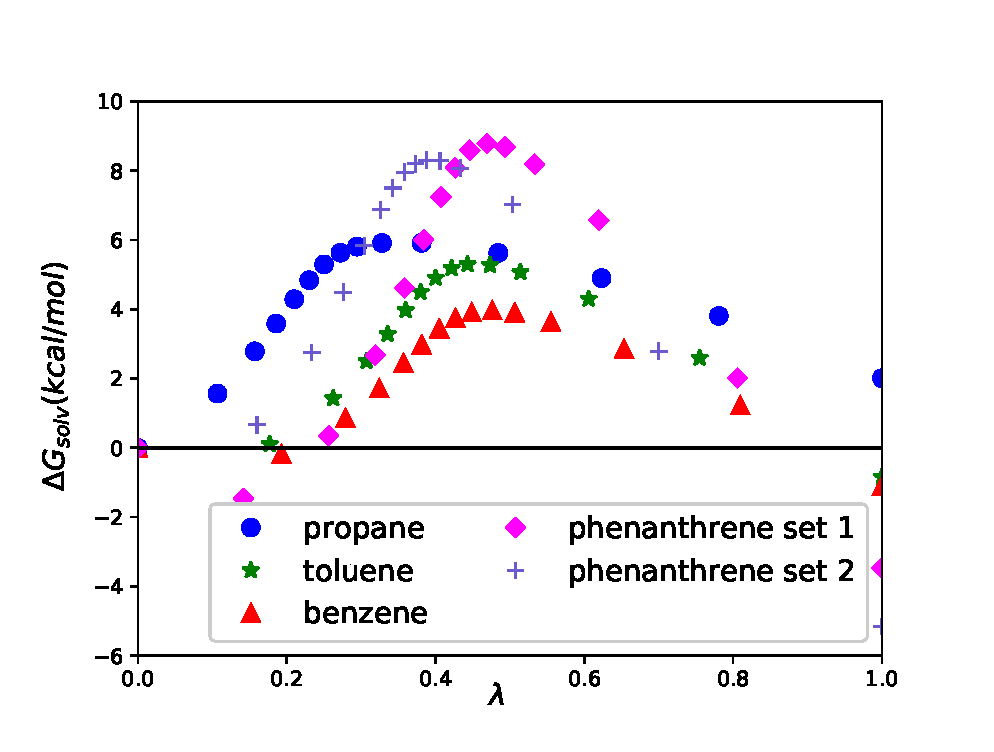
\includegraphics[width=1.0\linewidth]{Figures/waterartsets.eps}
		\caption{Representation of hydration free energies of different solutes calculated using the SAFT-$\gamma$ Mie force field. Each point on the graph represents the solvation free energy difference estimated with MBAR at each alchemical state.}
		\label{fig:water}
	\end{figure}
	
	\section{Conclusions}

	This study consisted in the calculation of solvation free energies of aromatic solutes in different solvents by using the SAFT-$\gamma$ Mie coarse-grained force field. Solvation free energy studies are mostly presented in the literature using water as a solvent and with all-atom force fields based on the Lennard-Jones potential. In contrast, in the present study, we provide data about the capability of a coarse-grained force field based on the Mie potential in calculating solvation free energies. Additionally, the solvation free energy estimations carried out here can help improve the SAFT-$\gamma$ Mie force field since these calculations are helpful in identifying errors and shortcomings in the modeling process. This force field uses the SAFT-VR Mie equation of state in its parameterization, which results in a relatively straightforward top-down method of obtaining parameters. Following this strategy, parameters for phenanthrene, which were not available in the original database of this force field, were obtained using vapor pressure data and the corresponding states parametrization.

	In order to perform expanded ensemble simulations, we optimized the set of coupling parameter states and their respective importance weights. The potential energies resulting from the expanded ensemble simulations then served as input to estimate solvation free energies with the MBAR method. The results for non-aqueous solvents had absolute deviations from the experimental data of less than 2.0 kcal/mol, except for anthracene/1-octanol. Additionally, the parameters of phenanthrene estimated with the corresponding states methodology resulted in solvation free energies with smaller absolute deviations to the experimental data. We also observed the geometry effect on the free energy as a function of the coupling parameter $\lambda$ - larger molecules exhibited steeper curves for small $\lambda$ values and yielded larger absolute deviations. The influence of carbon dioxide on the solvation free energy of phenanthrene in toluene was found to be negligible according to the SAFT-$\gamma$ Mie force field. Hydration free energy calculations required the use of relatively large values of $k_{ij}$ to produce satisfactory results.
	This necessity of one additional parameter is probably due to the lack of a term to account for hydrogen bonds in the EoS on which this force field is based and due to problems associated with the coarse-graining of water molecules. The results obtained with $k_{ij}$ estimated with MD and solvation free energy data were satisfactory, with absolute deviations from experimental data being smaller than the ones obtained elsewhere with the GAFF and ELBA force fields.

	Overall, the SAFT-$\gamma$ Mie force field proved to be a suitable model to represent the solvation phenomenon in non-aqueous solvents. It correctly described solvation free energies of asphaltene-like solutes dissolved in hexane, toluene, and 1-octanol. However, the calculation of hydration free energies required the use of a binary interaction parameter estimated with MD output, which increased the simulation time significantly. This fact evidenced flaws in the methodology used by the SAFT-$\gamma$ force field and raised questions about the practicality of this model for hydration free energy calculations. Nevertheless, the SAFT-$\gamma$ Mie force field for water used here does not predict freezing at room temperature as other force fields do, which is essential for reliable hydration free energy calculations, and the use of one average parameter resulted in hydration free energies compatible with the experimental data.
	Therefore, it would be relevant to test whether the binary interaction parameter estimated here for aromatic solutes can be transferred to hydration free energy calculations of other aromatic substances.

	\section*{Acknowledgements}
	
	The authors acknowledge the financial support provided by Petrobras (project code CENPES 17.564). They are also grateful to Prof. Bruno Horta (IQ/UFRJ) for his helpful comments and suggestions.
	
	\section*{Appendix A. Supplementary Data}
	
	Supplementary data related to this article can be found at fpe-supp-material.pdf.
	
	\section*{References}
	
	\bibliography{fpe-paper}
	
\end{document}
